\chapter{Singleton Pattern}

\section{Định nghĩa}
Singleton Pattern là một trong những mẫu Design Pattern đơn giản nhất trong Java.\\
Trong design pattern, mẫu thiết kế Singleton Pattern được dùng để đảm bảo chỉ có duy nhất một instance trong một class, và class đó sẽ cung cấp phương thức toàn cục để truy cập đến thực thể đó

\section{Mục đích sử dụng}
Khi cần một đối tượng chính xác để điều phối hành động trên toàn hệ thống. Các hệ thống vận hành hiệu quả hơn khi chỉ có một đối tượng tồn tại hoặc hạn chế sự khởi tạo cho một số lượng đối tượng nhất định. Thuật ngữ này xuất phát từ khái niệm toán học của một singleton.

\section{Singleton Pattern trong thực tế}
Dưới đây là một số trường hợp sử dụng của Singleton Pattern thường gặp:
\begin{itemize}
\item	Vì class dùng Singleton chỉ tồn tại 1 Instance (thể hiện) nên nó thường được dùng cho các trường hợp giải quyết các bài toán cần truy cập vào các ứng dụng như: Shared resource, Logger, Configuration, Caching, Thread pool, …\\
\item	Một số design pattern khác cũng sử dụng Singleton để triển khai: Abstract Factory, Builder, Prototype, Facade,…\\
\item	Đã được sử dụng trong một số class của core java như: java.lang.Runtime, java.awt.Desktop.
\end{itemize}
\section{Mô hình cấu trúc}
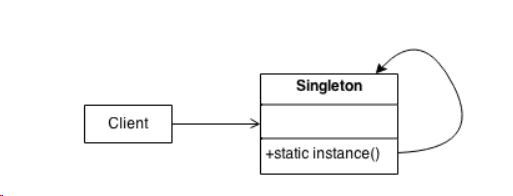
\includegraphics{GALLEYS/images/chapter1/diagram01}
\begin{multicols}{2}
\vspace{-20pt}
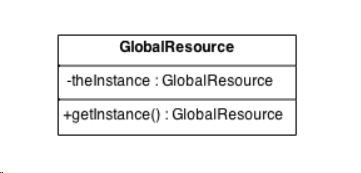
\includegraphics{GALLEYS/images/chapter1/diagram2}
\textbf{Mô tả đôi nét:} để đảm bảo chỉ có duy nhất một instance trong một class thì ta tạo ra một construct mang thuộc tính private.\\
Nhưng nó nảy sinh ra một vấn đề là private chỉ có thể được khai báo ở nội bộ của class đó.
\end{multicols}
Ta có thể vừa khắc phục vấn đề chỉ có một instance bằng phương thức public static(phương thức tĩnh) vì thành phần static chỉ có thể gọi một lần. Cụ thể :\\\\
- Lớp Singleton khai báo static method getInstance() trả về cùng một thể hiện của lớp riêng của nó.\\
- Constructor của Singleton phải là private. Gọi phương thức getInstance() là cách duy nhất để lấy đối tượng Singleton.
Chúng Ta sẽ đi sâu hơn vào ví dụ để tìm hiểu:\\
\begin{multicols}{2}
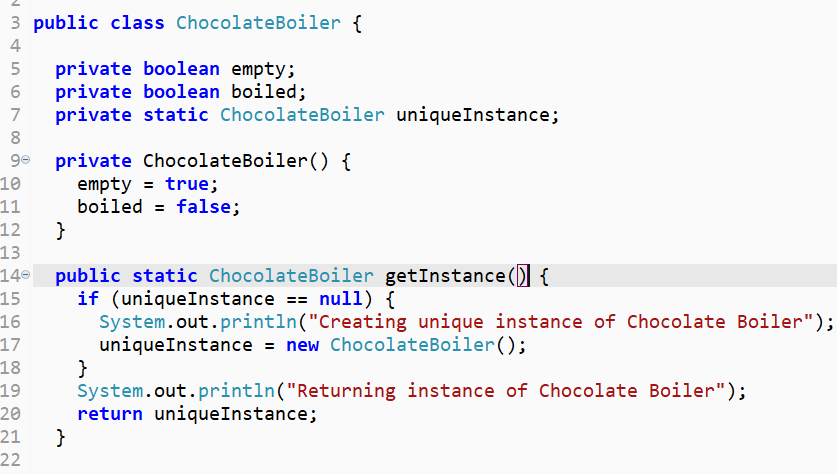
\includegraphics[height=0.23\textheight]{GALLEYS/images/chapter1/images1s}

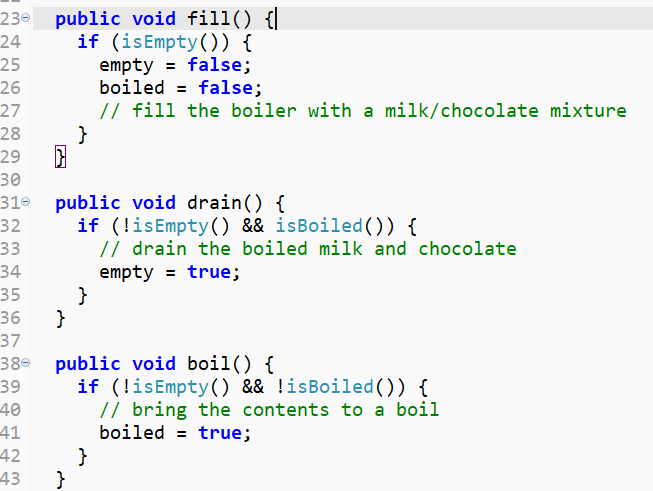
\includegraphics[height=0.25\textheight]{GALLEYS/images/chapter1/images1f}
\end{multicols}
+) trong ví dụ về nồi hơi chocolate ở trên:\\
Ta có một construct với phạm vi là private (private ChocolateBoiler()) và một đối tượng singleton sẽ không cần phải khởi tạo mà chỉ cần gọi đến phương thức tĩnh getInstance(). Đặc biệt việc khởi tạo đối tượng thông qua phương thức tĩnh getInstance() chỉ được thực hiện 1 lần.\\
Đây là kết quả:\\
\begin{center}
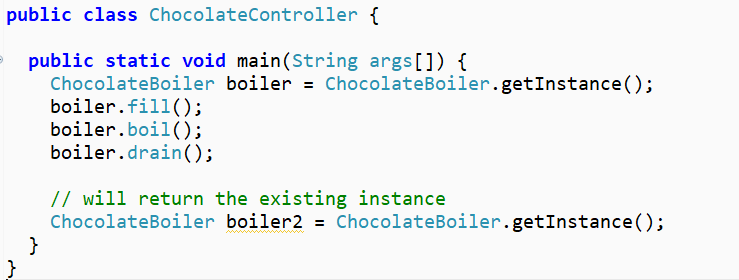
\includegraphics[scale=0.75]{GALLEYS/images/chapter1/images2}\\
\vspace{1cm}
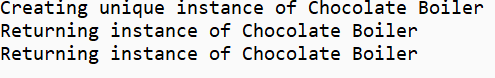
\includegraphics{GALLEYS/images/chapter1/images3}
\end{center}
Có thể thầy chỉ có duy nhất một đối tượng được khởi tạo trong lớp dù có khai báo bao nhiêu lần đi nữa.




